\subsection{Grafikon kirajzoló - Flot}

	\begin{figure}[h]
	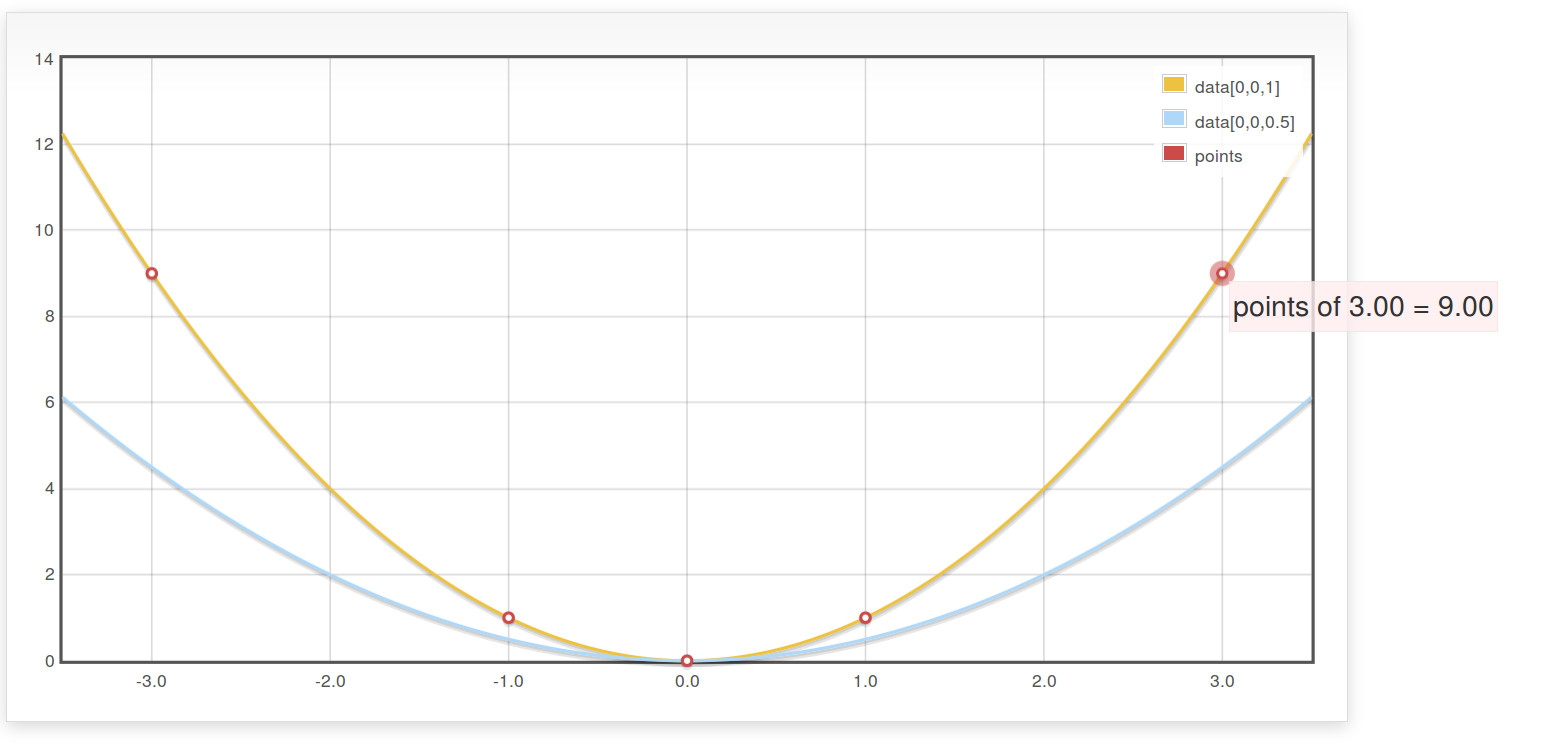
\includegraphics[width=13cm]{pics/plot}
	\centering
	\caption{Grafikon kirajzoló\label{fig:plot}}

	\end{figure}
		A Grafikon megjelenítéséhez a Flot-ot használom. Ez egy jQuery-s könyvtár, melyben egyszerűen és látványosan lehet grafikonokat kirajzolni. A forrás a "WebPage/source/flot-8.0.2" mappában érhető el.
		HTML fájlban egy egyszerű "DIV"-ként jelenik meg, melyet aztán a JavaScript tölt meg tartalommal.
				\begin{minted}{html}
	<div id=\"resultplot\" class=\"demo-placeholder\"></div>
			\end{minted}
		A JavaScript-ben hivatkozhatunk erre a "DIV"-re, majd az adatok és a típusok segítségével alábbi módon hivatkozhatjuk meg: 
		\begin{minted}{javascript}
	    var placeholder = $("#resultplot");
	    var plot = $.plot(placeholder, flot_data, type);
		\end{minted}
		A paraméterezése a grafikon kirajzolónak az alábbi: 
		\begin{description}
			\item[placeholder] \hfill \\ 
	 			DIV hivatkozása
	 		 \item[type] \hfill \\ 
	 			Megjelenítendő grafikon típusa
	 			\newline
	 			A Flot sok lehetőséget nyújt a típusok kiválasztására, és ezekre való példákból megalkottam a saját típusomat mely a következőket tartalmazza egy objektumban:
		 		
		 		\begin{verbatim}
		 			series: { line: { show: true } } 
		 		\end{verbatim}
				Beállítjuk hogy a vonalakat jelenítse meg. Ekkor a pontokat is megjeleníti, a többi beállítás függvényében.
		 		
		 		\begin{verbatim}
					xaxis: { zoomRange: [0.1, 1], panRange: [-1000, 1000] }
					yaxis: { zoomRange: [0.1, 100], panRange: [-1000, 1000] }
		 		\end{verbatim} 
		 		X és Y koordinátákon nagyítás és mozgatási beállítások interaktívvá állítása
			 	\begin{verbatim}
			 		grid: { hoverable: true, clickable: true }
			 	\end{verbatim} 
			 	Ezeket a tulajdonságokat használjuk arra hogy felvegyünk új pontokat.\newline
			 	Emellett ha ráviszem az egeret az egyik pontra, megmutatja a pont koordinátáját, és értékeit, és hogy melyik ponthalmazon van.
			 	\begin{verbatim}
			 		zoom: { interactive: true}, pan: { interactive: true }
			 	\end{verbatim} 
			 	Nagyítás és kattintással mozgatás engedélyezése. \newline
				Ennek a beépítésével is foglalkoztam, de a kattintás sajnos nem egyeztethető könnyen össze a pont figyeléssel, valamint a beépítés után lassú lett, és akadozott a felület, így végül az interaktivitását külső komponensekkel(inputokkal) oldottam meg.

	 		\item[flot\_data] \hfill \\ 
	 		A tényleges adathalmazokat tartalmazó tömb, melyben az egyes adatokról egyéni információkat is tartalmazza.\newline
	 		\begin{description}
				\item[data] \hfill \\ 
				Pontok halmaza, melyeket megjelenítünk\newline
				[x, y] pontokból álló tömb\newline
				Polinom esetén is ezt használjuk, ezért a polinom behelyettesített értékeit adjuk itt meg. Amikor az egérrel felé megyünk ezeket a pontokat fogja megjeleníteni.
				\item[label] \hfill \\ 
				Adathalmaz elnevezése, ezt láthatjuk amikor az egérrel a pont felé visszük az egeret, valamint a színek-elnevezések össze párosításánál is segít.
				\item[points] \hfill \\ 
				Ha pontokat kívánunk megjeleníteni, akkor ezt a kapcsolót kell alkalmazni.
				\item[lines] \hfill \\ 
				Ha a pontokból alkotott vonalat kívánunk látni, akkor ezt a kapcsolót kell alkalmazni. Ezt használjuk a polinom megjelenítéséhez.
			\end{description}
	 		\begin{minted}{javascript}
		var example_datas = [{
			data: d4,
			label: "neved4",
			lines: { show: true }
		}, {
		    data: d3,
			label: "neved43"
		    points: { show: true }
		}];
			\end{minted}
		\end{description}
\subsection{Http szerver}
	A http szerver gyakorlatilag 2 példából lett megvalósítva:
	"httpServer leírása TODO"
\subsection{Ping-pong Node figyelő}
	"pingPong TODO: pidWatcher mit csinál"
\subsection{mochi json}
	Struktúra kezelő "structHandler"

\subsection{Erlang modul C++-ban : erl\_nif}